  \documentclass[final]{beamer} % beamer 3.10: do NOT use option hyperref={pdfpagelabels=false} !
  %\documentclass[final,hyperref={pdfpagelabels=false}]{beamer} % beamer 3.07: get rid of beamer warnings
  \mode<presentation> {  %% check http://www-i6.informatik.rwth-aachen.de/~dreuw/latexbeamerposter.php for examples
    \usetheme{Berlin}    %% you should define your own theme e.g. for big headlines using your own logos 
  }
  \usepackage[english]{babel}
  \usepackage[latin1]{inputenc}
  \usepackage{amsmath,amsthm, amssymb, latexsym}


  %\usepackage{times}\usefonttheme{professionalfonts}  % times is obsolete
  %\usefonttheme[onlymath]{serif}
  %\boldmath
  %\usepackage{arev}
  %\renewcommand{\sfdefault}{arev}

\usepackage[T1]{fontenc}
\usepackage{lmodern}


  \usepackage[orientation=landscape,size=a0,scale=1.4]{beamerposter}                       % e.g. for DIN-A0 poster
  %\usepackage[orientation=portrait,size=a1,scale=1.4,grid,debug]{beamerposter}                  % e.g. for DIN-A1 poster, with optional grid and debug output
  %\usepackage[size=custom,width=200,height=120,scale=2,debug]{beamerposter}                     % e.g. for custom size poster
  %\usepackage[orientation=portrait,size=a0,scale=1.0,printer=rwth-glossy-uv.df]{beamerposter}   % e.g. for DIN-A0 poster with rwth-glossy-uv printer check
  % ...
  %
  \title[Fancy Posters]{Making Really Fancy Posters with \LaTeX}
  \author[Dreuw \& Deselaers]{Philippe Dreuw and Thomas Deselaers}
  \institute[RWTH Aachen University]{Human Language Technology and Pattern Recognition,RWTH Aachen University}
  \date{Jul. 31th, 2007}
  \begin{document}
  \begin{frame}{} 
  \begin{columns}[t]

%%%%%%%%%%%%%%%%%%%%%%%%%%%%%%%%%%%%%%%%%%%%%%%%%%%%%%%%%%%%%%%%%%%%%%%%%%%%%%%
% First column

  \begin{column}{.3\linewidth}

    \begin{block}{\large EXO-200}

      \begin{columns}
        \begin{column}{0.49\linewidth}
          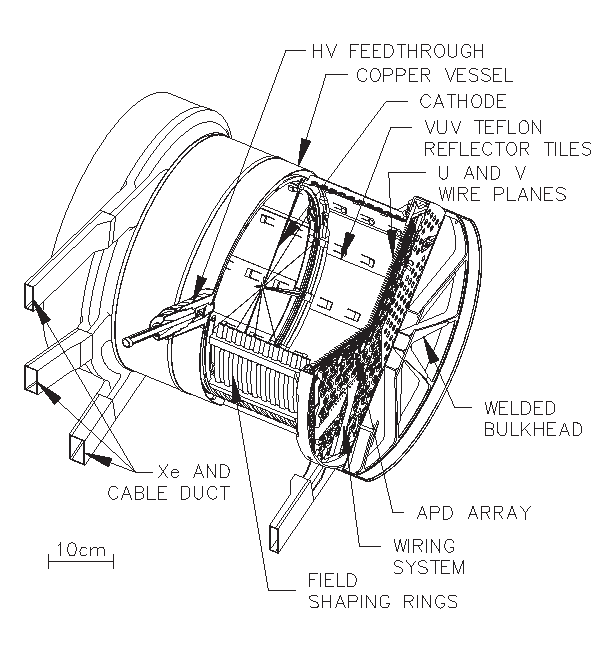
\includegraphics[keepaspectratio=true,width=\textwidth]{TPCSchematic.eps}
        \end{column}
        \begin{column}{0.49\linewidth}
          The EXO-200 TPC has 110 kg of liquid xenon, enriched to 80.6\% in $^{136}$Xe.  The xenon is continuously purified.  The TPC consists of a cathode in the middle and two anodes on the ends.
        \end{column}
      \end{columns}

      \begin{columns}
        \begin{column}{0.49\linewidth}
          We measure light and charge independently; combining them leads to much better resolution than either can provide individually.  Resolution is particularly important for us because small improvements in resolution can have a strong impact in thorium backgrounds from the 2615-keV gamma line of $^{208}$Tl.
        \end{column}
        \begin{column}{0.49\linewidth}
          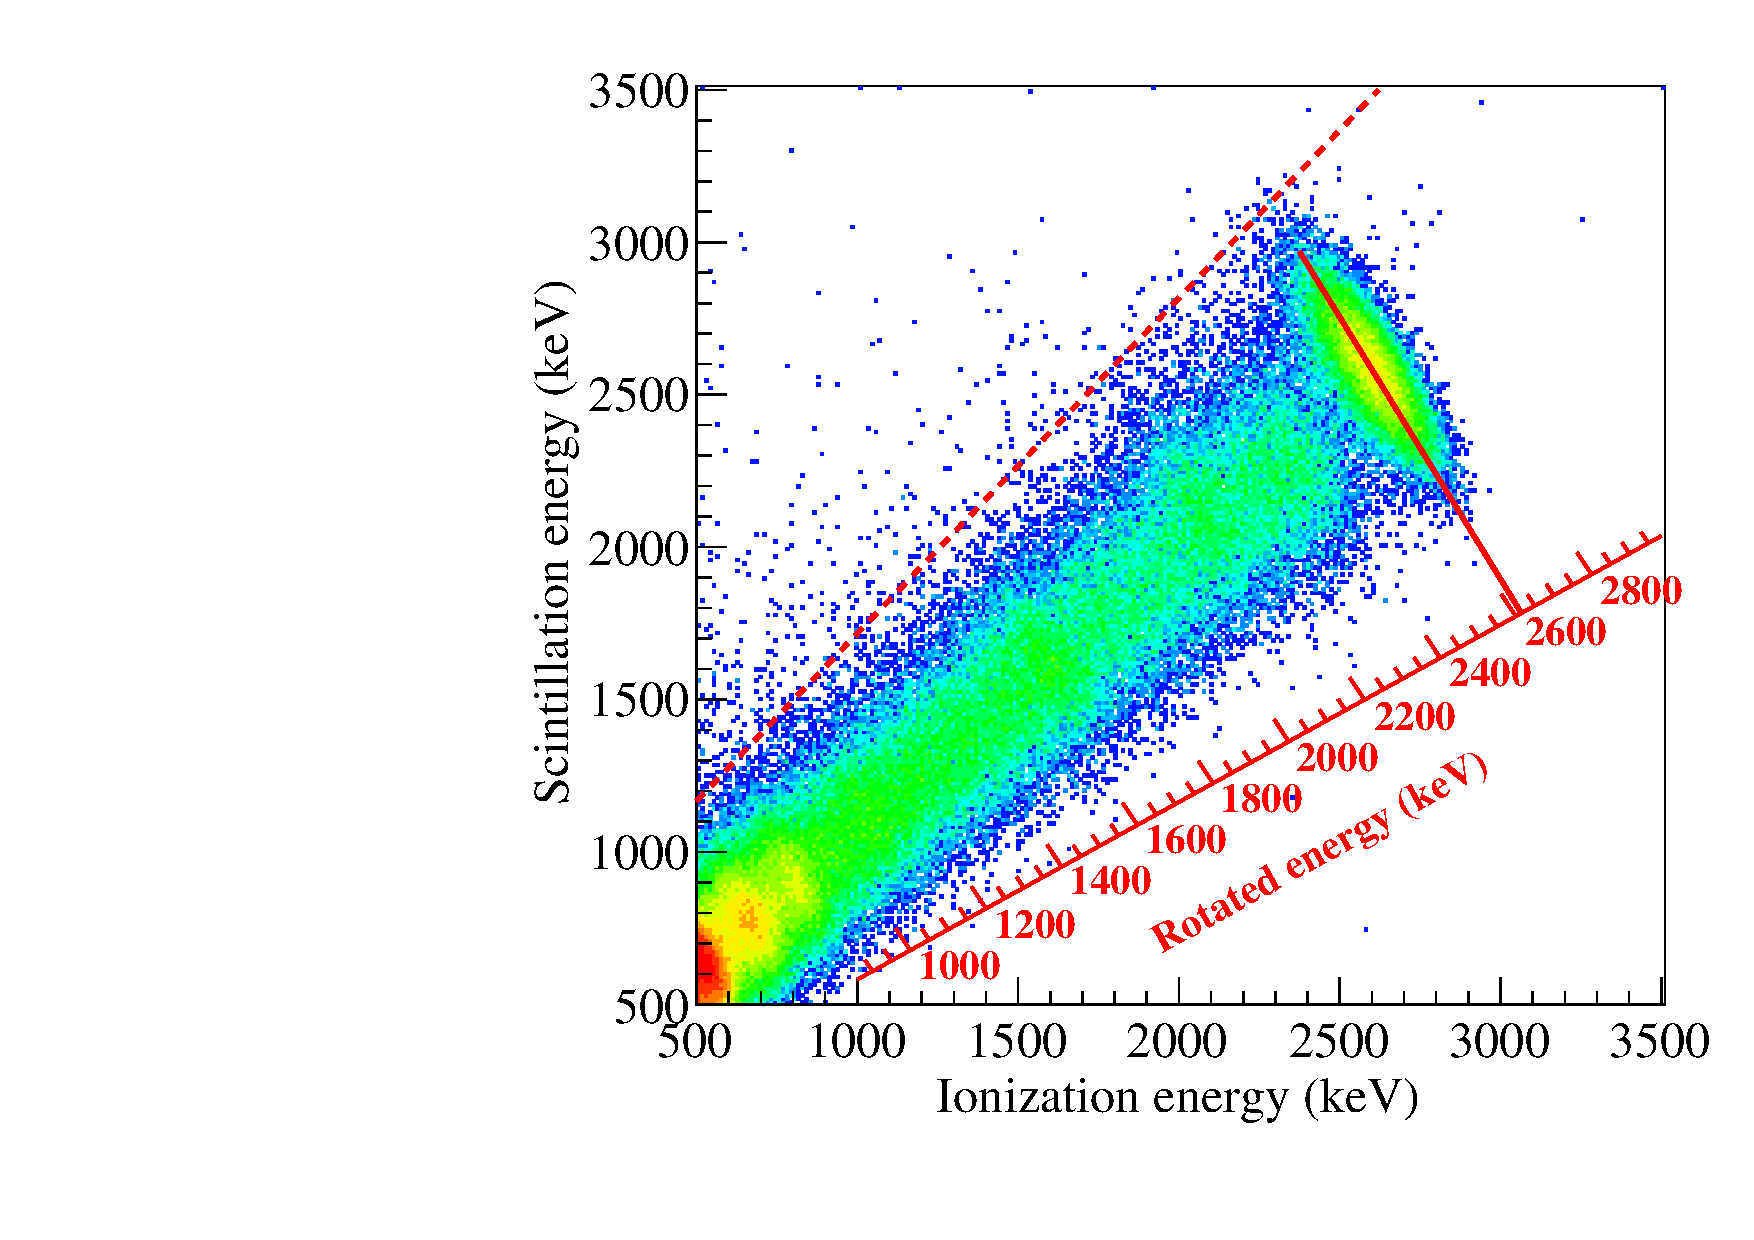
\includegraphics[keepaspectratio=true,width=\textwidth]{RotationTh2D_withCalibration.pdf}
        \end{column}
      \end{columns}

      \begin{columns}
        \begin{column}{0.49\linewidth}
          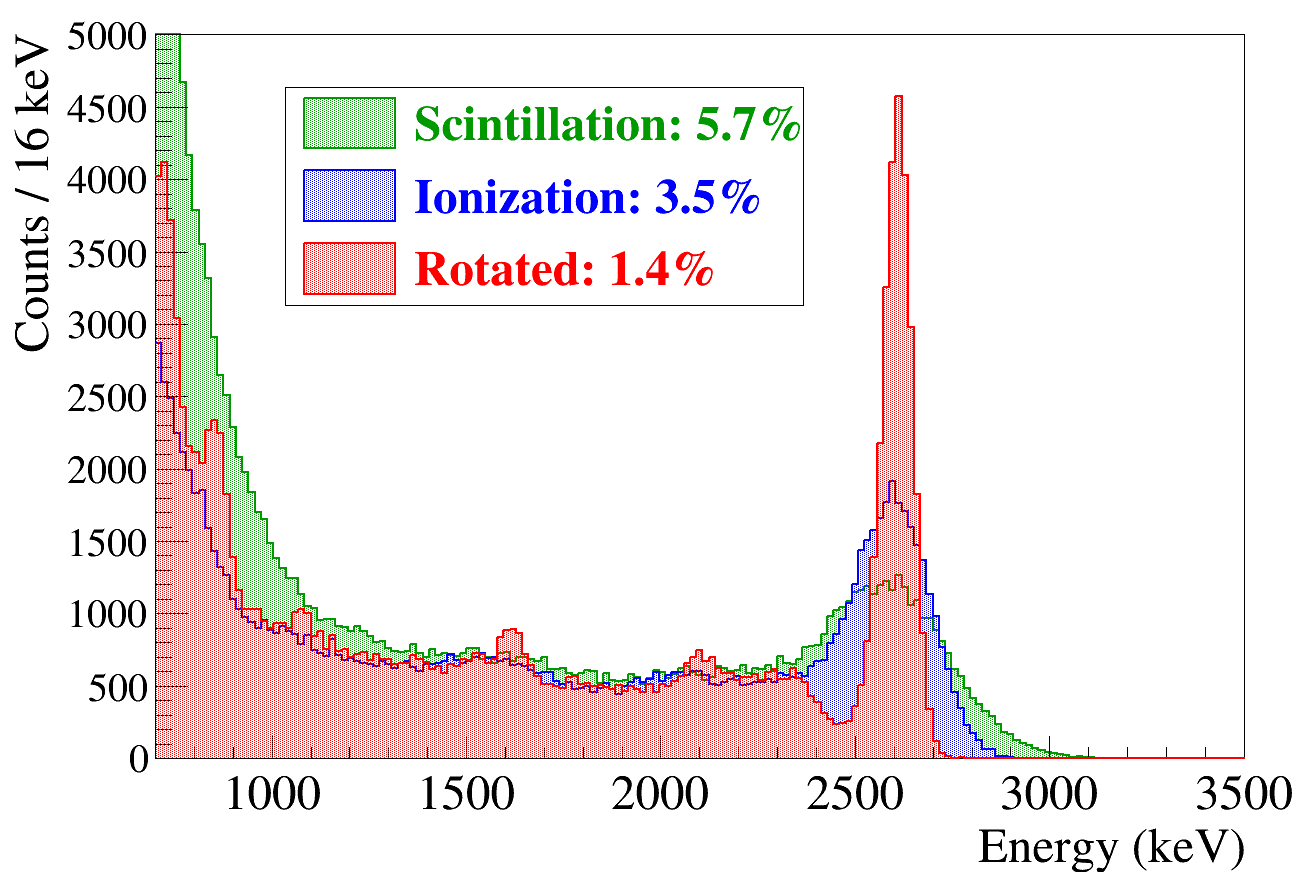
\includegraphics[keepaspectratio=true,width=\textwidth]{RotationTh2D_ImprovementInResolution.png}
        \end{column}
        \begin{column}{0.49\linewidth}
          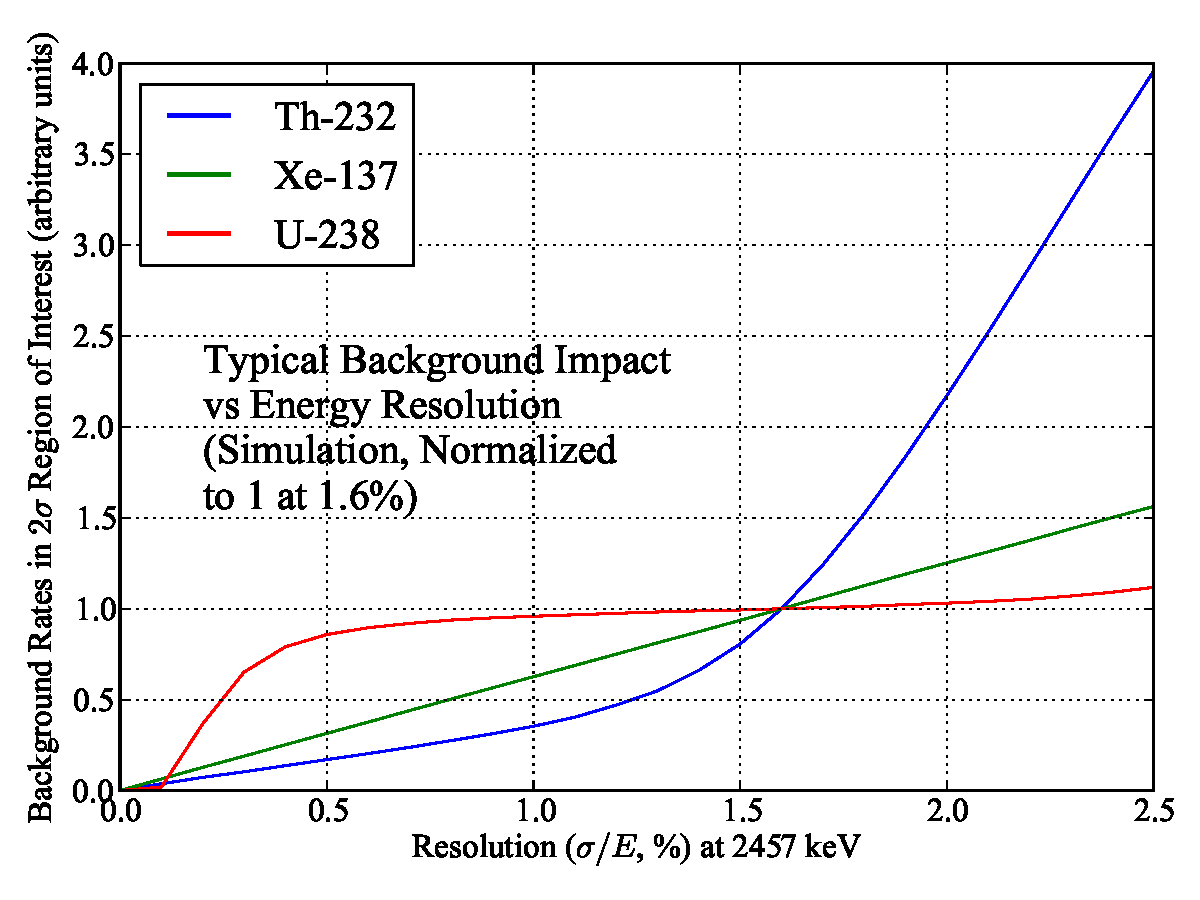
\includegraphics[keepaspectratio=true,width=\textwidth]{BackgroundsVsRes.pdf}
        \end{column}
      \end{columns}

    \end{block}

    \begin{block}{APD Noise Limits Resolution}
      \begin{columns}
        \begin{column}{0.49\linewidth}
          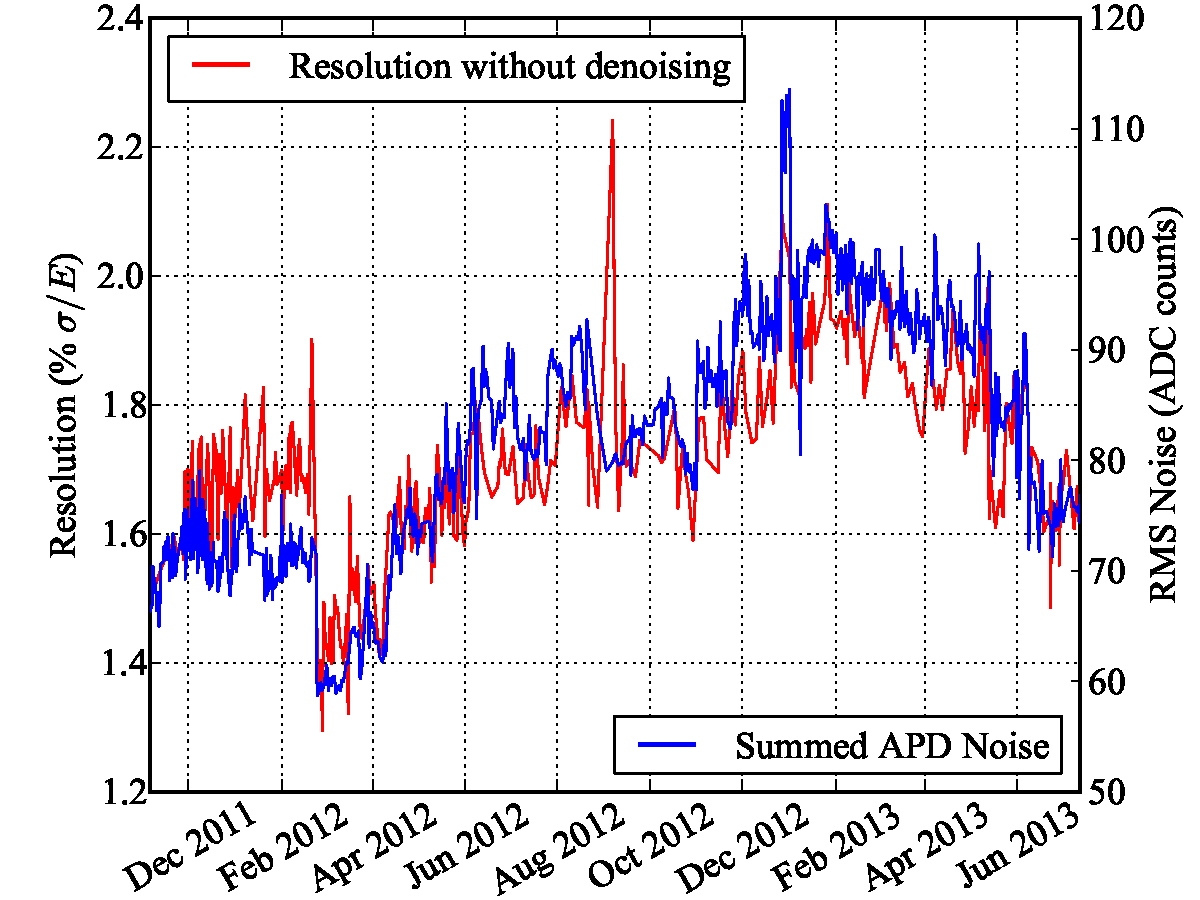
\includegraphics[keepaspectratio=true,width=\textwidth]{ResolutionAPDNoiseComparison.pdf}
         \end{column}
        \begin{column}{0.49\linewidth}
          Before denoising, energy resolution varies in time.  The resolution varies in the range 1.5-2.0\%, and the impact of thorium backgrounds depends strongly on resolution in this range.

We find that the resolution is highly correlated in time with RMS noise on the APDs.
        \end{column}
      \end{columns}

      \begin{columns}
        \begin{column}{0.49\linewidth}
           Noise on the APD waveforms is highly correlated across channels.

Individual channels are dominated by Poisson statistics on the signal; only when they are summed together does electronic noise become dominant.  We want a denoising scheme which simultaneously minimizes signal fluctuations and electronic noise.
         \end{column}
        \begin{column}{0.49\linewidth}
          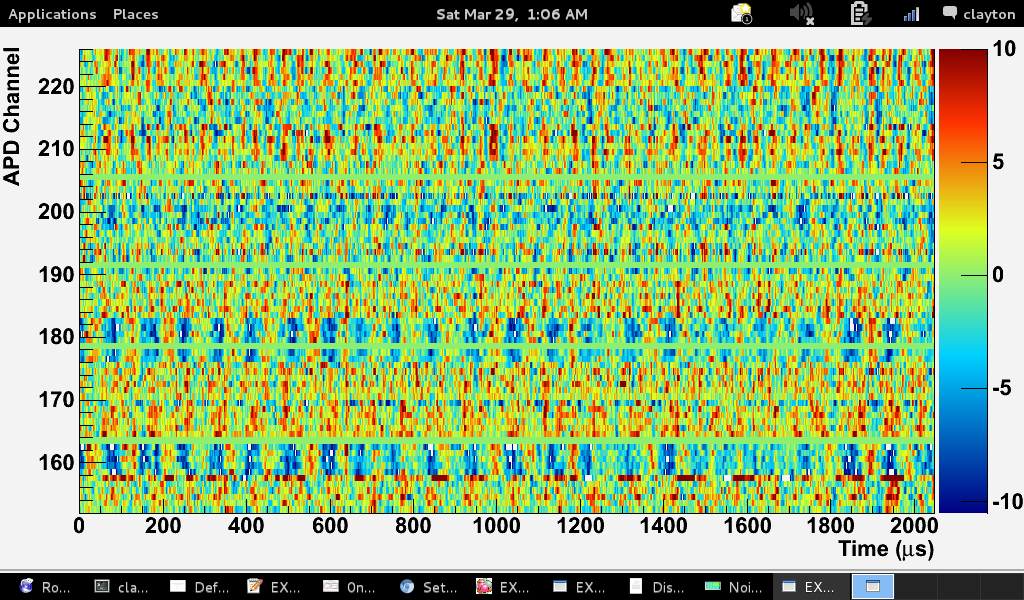
\includegraphics[keepaspectratio=true,width=\textwidth,clip=true,trim=0mm 12mm 0mm 10mm]{Run4705Ev2_noiseEventDisplay.png}
        \end{column}
      \end{columns}

    \end{block}

  \end{column}

%%%%%%%%%%%%%%%%%%%%%%%%%%%%%%%%%%%%%%%%%%%%%%%%%%%%%%%%%%%%%%%%%%%%%%%%%%%%%%%
% Second column

  \begin{column}{.3\linewidth}

    \begin{block}{\Huge \center APD Denoising in EXO-200 \\[\baselineskip]
                  \large by Clayton G. Davis \\
                  on behalf of the EXO-200 Collaboration}
    \end{block}

    \begin{block}{\large Model of a Waveform}
When there is one energy deposit in the xenon, the APD waveform $X_i[f]$ (in frequency space) on channel $i$ can be modeled:
\[X_i[f] = M_i Y_i[f] + N_i[f]\text{, where:}\]\\[-0.5\baselineskip]

\begin{itemize}
\item $Y_i[f]$ is the unit-magnitude template pulse for channel $i$.
\item $M_i$ is the pulse magnitude; it measures the scintillation energy, corrupted by Poisson fluctuations in photon statistics and gain.
\item $N_i[f]$ is the additive (electronic) noise on channel $i$.
\end{itemize}
    \end{block}

    \begin{block}{\large Characterizing the Lightmap}
We need a map of light yield versus deposit position for each channel to model the dependence of $M_i$ on energy.  Channels have time-dependent gain, so each channel $i$ needs a lightmap function $L_i(\vec{x}, t)$.  Very difficult to measure this empirically with limited source statistics.

However, we can make a simplifying assumption that $L_i$ is separable into a position-dependent and time-dependent component representing photon propagation through the detector and gain variations over time.  This lets us simplify:
\[L_i(\vec{x}, t) = R_i(\vec{x})S_i(t)\]
and we only need to empirically measure $R_i(\vec{x})$ and $S_i(t)$ for each channel -- much easier.

      \begin{columns}
        \begin{column}{0.49\linewidth}
           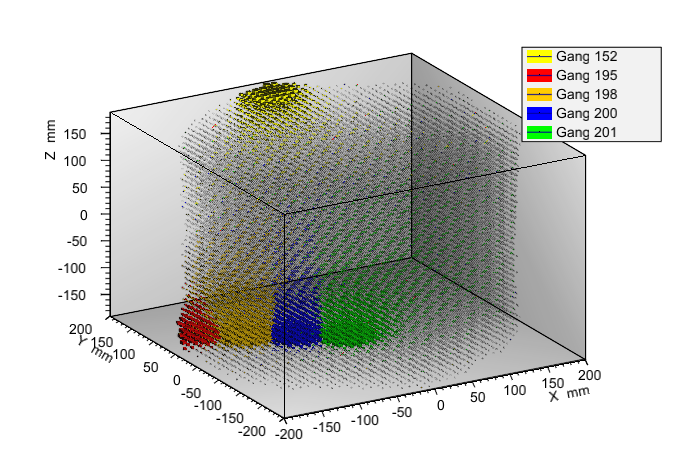
\includegraphics[keepaspectratio=true,width=\textwidth,clip=true,trim=15mm 10mm 10mm 10mm]{Lightmap_viz_zoom.png}
         \end{column}
        \begin{column}{0.49\linewidth}
          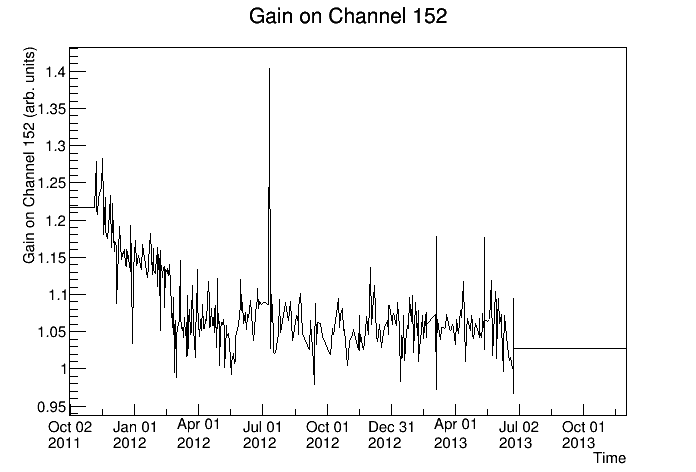
\includegraphics[keepaspectratio=true,width=\textwidth,clip=true,trim=5mm 0mm 20mm 15mm]{gainfunc_152.png}
        \end{column}
      \end{columns}
    \end{block}

    \begin{block}{\large Characterizing the Noise}
In general, we could characterize the noise to lowest order by measuring the correlations:
\[\left< N_i[f] N_j[g] \right>\text{ for each channel $i$, $j$ and frequency $f$, $g$.}\]
However, our noise is dominated by electronics and is relatively steady over short time periods; pairwise correlations will be zero when $f \ne g$.  So, we only need to characterize correlations:
\[\left< N_i[f] N_j[f] \right>\text{ for each channel $i$, $j$ and frequency $f$.}\]
Note that if we had significant dark current, we might be dominated by terms like $\left< N_i[f] N_i[g] \right>$ instead.

The beauty of a low-background detector is that it collects lots of noise, so measuring noise empirically is relatively easy.
    \end{block}

  \end{column}

%%%%%%%%%%%%%%%%%%%%%%%%%%%%%%%%%%%%%%%%%%%%%%%%%%%%%%%%%%%%%%%%%%%%%%%%%%%%%%%
% Third column

  \begin{column}{.3\linewidth}

    \begin{block}{\large Fontsizes}
      \centering
      {\tiny tiny}\par
      {\scriptsize scriptsize}\par
      {\footnotesize footnotesize}\par
      {\normalsize normalsize}\par
      {\large large}\par
      {\Large Large}\par
      {\LARGE LARGE}\par
      {\veryHuge veryHuge}\par
      {\VeryHuge VeryHuge}\par
      {\VERYHuge VERYHuge}\par
    \end{block}

  \end{column}

%%%%%%%%%%%%%%%%%%%%%%%%%%%%%%%%%%%%%%%%%%%%%%%%%%%%%%%%%%%%%%%%%%%%%%%%%%%%%%%

  \end{columns}
  \end{frame}
  \end{document}
